%%%%%%%%%%%%%%%%%%%%%%% file template.tex %%%%%%%%%%%%%%%%%%%%%%%%%
%
% This is a general template file for the LaTeX package SVJour3
% for Springer journals.          Springer Heidelberg 2010/09/16
%
% Copy it to a new file with a new name and use it as the basis
% for your article. Delete % signs as needed.
%
% This template includes a few options for different layouts and
% content for various journals. Please consult a previous issue of
% your journal as needed.
%
%%%%%%%%%%%%%%%%%%%%%%%%%%%%%%%%%%%%%%%%%%%%%%%%%%%%%%%%%%%%%%%%%%%
%
% First comes an example EPS file -- just ignore it and
% proceed on the \documentclass line
% your LaTeX will extract the file if required
\begin{filecontents*}{example.eps}
%!PS-Adobe-3.0 EPSF-3.0
%%BoundingBox: 19 19 221 221
%%CreationDate: Mon Sep 29 1997
%%Creator: programmed by hand (JK)
%%EndComments
gsave
newpath
  20 20 moveto
  20 220 lineto
  220 220 lineto
  220 20 lineto
closepath
2 setlinewidth
gsave
  .4 setgray fill
grestore
stroke
grestore
\end{filecontents*}
%
\RequirePackage{fix-cm}
%
%\documentclass{svjour3}                     % onecolumn (standard format)
%\documentclass[smallcondensed]{svjour3}     % onecolumn (ditto)
\documentclass[smallextended]{svjour3}       % onecolumn (second format)
%\documentclass[twocolumn]{svjour3}          % twocolumn
%
\smartqed  % flush right qed marks, e.g. at end of proof
%
\usepackage{graphicx}
%
% \usepackage{mathptmx}      % use Times fonts if available on your TeX system
%
% insert here the call for the packages your document requires
%\usepackage{latexsym}
% etc.
%
% please place your own definitions here and don't use \def but
% \newcommand{}{}
%
% Insert the name of "your journal" with
% \journalname{myjournal}
%
\usepackage{amsmath}
\usepackage{mathrsfs}
\DeclareMathAlphabet{\mathpzc}{OT1}{pzc}{m}{it}

\usepackage{amssymb}
\usepackage{epstopdf}
\usepackage{mathtools}


\usepackage{fouriernc}
\usepackage{float}

\usepackage{algorithm}
\usepackage[noend]{algpseudocode}

\usepackage{array}

\newtheorem{hypothesis}{Hypothesis}
%\newtheorem{property}{Property}
\newtheorem{fact}{Fact}
\newtheorem{formula}{Formula}

\usepackage{pifont}% http://ctan.org/pkg/pifont
\newcommand{\cmark}{\ding{51}}%
\newcommand{\xmark}{\ding{55}}%


\newcommand{\aj}    {\mbox{\it AJ}}
\newcommand{\bc}    {\mbox{\it BC}}
\newcommand{\bd}    {\mbox{\it BD}}
\newcommand{\br}    {\mbox{\it BR}}
\newcommand{\bt}    {\mbox{\it BT}}
\newcommand{\hb}    {\mbox{\it HB}}
\newcommand{\hi}    {\mbox{\it HI}}
\newcommand{\ih}    {\mbox{\it IH}}
\newcommand{\wc}    {\mbox{\it WC}}
\newcommand{\wcd}   {\mbox{\it WD}}
\newcommand{\wl}       {\mbox{\it WL}}
\newcommand{\wo}     {\mbox{\it WO}}
\renewcommand{\wr}  {\mbox{\it WR}}
\newcommand{\wt}    {\mbox{\it WT}}
\newcommand{\bu}    {\mbox{\it BU}}
\newcommand{\wh}    {\mbox{\it WH}}
\newcommand{\bh}    {\mbox{\it BH}}
\newcommand{\hlt}    {\mathpzc{H}}

\newcommand\defeq{\stackrel{\mathclap{\tiny\mbox{def}}}{=}}
\DeclarePairedDelimiter{\ceil}{\lceil}{\rceil}


\begin{document}

\title{Best-case response times and jitter analysis of real-time tasks under fixed priority scheduling with preemption thresholds%\thanks{Grants or other notes
%about the article that should go on the front page should be
%placed here. General acknowledgments should be placed at the end of the article.}
}
%\subtitle{Do you have a subtitle?\\ If so, write it here}

\titlerunning{Best-case response times and jitter analysis of real-time tasks under FPTS}        % if too long for running head

\author{H.J. Rivera-Verduzco         \and
        Reinder J. Bril %etc.
}

%\authorrunning{Short form of author list} % if too long for running head

\institute{Hector J. Rivera-Verduzco and Reinder J. Bril \at
              Eindhoven University of Technology \\
%              Tel.: +123-45-678910\\
%              Fax: +123-45-678910\\
              \email{h.j.rivera.verduzco@student.tue.nl, r.j.bril@tue.nl}           %  \\
%             \emph{Present address:} of F. Author  %  if needed
%           \and
%           S. Author \at
%              second address
}

\date{Received: date / Accepted: date}
% The correct dates will be entered by the editor


\maketitle

\begin{abstract}
Insert your abstract here. Include keywords, PACS and mathematical
subject classification numbers as needed.
\keywords{best-case \and response time analysis \and preemption thresholds \and jitter analysis}
% \PACS{PACS code1 \and PACS code2 \and more}
% \subclass{MSC code1 \and MSC code2 \and more}
\end{abstract}

\section{Introduction} \label{intro}
Your text comes here. Separate text sections with

\section{Real-time scheduling model } \label{sec:model}

In this section, we present the basic real-time scheduling model for FPPS and FPTS along with some related notion that we use throughout this paper.

\subsection{Basic model for FPPS}
We assume a single processor and a set $\mathpzc{T}$ of $n$ independent periodic tasks $\tau_1,\tau_2,...,\tau_n$ with unique and fixed priorities $\pi_{1}$, $\pi_{2},...,\pi_{n} \in \mathbb{N^{+}}$. At any moment in time, the processor executes the task with the highest priority that has work pending. We also assume that tasks are given in order of decreasing priority, i.e. $\tau_1$ has the highest priority whereas $\tau_n$ has the lowest priority. A higher priority is represented by a higher value, i.e. $\pi_1 > \pi_2 >...>\pi_n$.

Each task $\tau_i$ generates an infinite sequence of jobs $\iota_{i,k}$ with $k\in \mathbb{Z}$. The inter arrival times of $\tau_i$ are determined by a (fixed) \textit{period} $T_i \in \mathbb{R^{+}}$ and an (absolute) \textit{activation jitter} $\aj_i \in \mathbb{R^{+} \cup \{0\} }$, where $\aj_i < T_i$. Furthermore, each task is characterized by a \textit{worst-case computation time} $\wc_i \in \mathbb{R^{+}}$, a \textit{best-case computation time} $\bc_i \in \mathbb{R^{+}}$, where $\bc_i \leq \wc_i$, a \textit{phasing} $\phi_i \in \mathbb{R}$, a (relative) \textit{worst-case deadline} $\wcd_i \in \mathbb{R^{+}}$, and a (relative) \textit{best-case deadline} $\bd_i \in \mathbb{R^{+}}\cup \{0\}$, where $\bd_i \leq \wcd_i$. We assume arbitrary deadlines; hence, deadline $\wcd_i$ may be smaller than, equal to, or larger than period $T_i$. The set of phasings $\phi_i$ is termed the phasing $\phi$ of the task-set $\mathpzc{T}$. We also assume that we do not have control over the initial phasing of the system, i.e. arbitrary phasings. Finally, we assume that tasks do not suspend themselves, jobs do not start before the completion of previous jobs of the same task, and the overhead of context switching and task scheduling is ignored.

Throughout this paper, we sometimes use $C_i$ to express the \textit{computation time} of a task $\tau_i$ when $\bc_i=\wc_i$. In addition, note that the activations of $\tau_i$ do not necessarily take place strictly periodically. Instead, they take place in an interval of length $AJ_i$ that repeats with period $T_i$. In general, the activation time $a_{i,k}$ of a job of $\tau_i$ satisfies
\begin{align}
\varphi_i + kT_i \leq a_{i,k} \leq 	\varphi_i + kT_i + \aj_i.
\end{align}
A task with activation jitter equal to zero is termed a \textit{strictly periodic} task.

\subsection{Refined model for FPTS}
For FPTS, each task $\tau_i$ has an additional property called \textit{preemption threshold} denoted by $\theta_i \in \mathbb{N^+}$, where $\pi_1 \geq \theta_i \geq \pi_i$. A task $\tau_i$ can be preempted by a higher priority task $\tau_h$ if and only if $\pi_h > \theta_i$. FPPS is a special case of FPTS when the preemption threshold of each task is equal to its priority, i.e. when $\forall_{1\leq i \leq n}\theta_i = \pi_i$. Furthermore, when all the preemption thresholds are set to the highest priority, FPTS becomes equivalent to FPNS, i.e. when $\forall_{1\leq i \leq n}\theta_i = \pi_1$.

\subsection{Derived notions}

The \textit{response time} $R_{i,k}$ of a job $\iota_{i,k}$ is defined as the time elapsed between its (absolute) \textit{finalization time} $f_{i,k}$ and (absolute) \textit{activation time} $a_{i,k}$, i.e. $R_{i,k}=f_{i,k}-a_{i,k}$. The \textit{relative finalization time} $F_{i,k}$ of a job $\iota_{i,k}$ is defined relative to the start of
the interval in which $\iota_{i,k}$ is activated, i.e. $F_{i,k}=f_{i,k}-(\varphi_i+kT_i)$. The (absolute) \textit{start time} $s_{i,k}$ is the time at which job $k$ of $\tau_i$ starts its execution. Furthermore, the \textit{relative start time} $S_{i,k}$ is the start time relative to the activation of a job, i.e. $S_{i,k}=s_{i,k}-a_{i,k}$. Finally, we define the \textit{hold time} $H_{i,k}$ as the time elapsed between the start of a job and its finalization, this is expressed as $H_{i,k}=f_{i,k}-s_{i,k}$. In general, under this model, it always holds that $R_{i,k}=S_{i,k}+H_{i,k}$. Figure \ref{fig:taskmodel} shows the basic task model with these notions. It is worth noting that, whereas $F_{i,k} = R_{i,k}$ holds for a strictly periodic task $\tau_i$, the following relation holds in general
\begin{align}
	\aj_i + R_{i,k} \geq F_{i,k} \geq R_{i,k}.
\end{align}

\begin{figure}[t]
	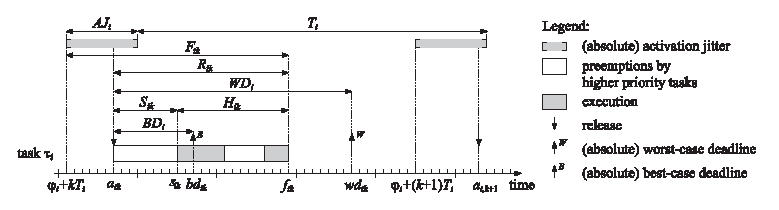
\includegraphics[width=1\linewidth]{figures/model2}
	\caption{Basic model for a periodic task $\tau_i$ with (absolute) activation jitter $\aj_i$.}
	\label{fig:taskmodel}
\end{figure}

The \textit{worst-case response time} $\wr_i$ and the \textit{best-case response time} $\br_i$ of a task $\tau_i$ are defined as the longest and the shortest response times of its jobs respectively, i.e.
\begin{align*}
	\wr_i \defeq \text{sup}_{\phi,k} R_{i,k}(\phi),  \text{\hspace{7mm}}
	\br_i \defeq \text{inf}_{\phi,k} R_{i,k}(\phi),
\end{align*}
where $R_{i,k}(\phi)$ denotes a dependency of the response time $R_{i,k}$ on the phasing $\phi$.

As is common for critical real-time applications, we assume that deadlines are hard, i.e. each
job of a task must be completed at or after its best-case deadline and at or before its worst-case deadline. Therefore, a set $\mathpzc{T}$ of $n$ periodic tasks is said to be schedulable if and only if
\begin{align}
	\displaystyle\mathop{\forall}_{1 \leq i \leq n}(\bd_i\leq \br_i \land \wr_i \leq \wcd_i).
\end{align}

Finally, we define the \textit{worst-case utilization} $U^{\mathpzc{T}}$ and the \textit{best-case utilization} $\bu^{\mathpzc{T}}$ as the worst and best fraction of the  processor time spent on the execution of $\mathpzc{T}$ respectively \cite{LL73}, i.e.
\begin{align*}
	U^{\mathpzc{T}} \defeq \sum_{1\leq i \leq n} \frac{\wc_i}{T_i}, \text{\hspace{10mm}} \bu^{\mathpzc{T}} \defeq \sum_{1\leq i \leq n} \frac{\bc_i}{T_i}.
\end{align*} 

\section{Recap of the existing analysis}

\subsection{Best-case response time analysis for FPPS}

\subsection{Best-case response time analysis for FPTS without jitter??}
Add here facts and bcrt analysis of RTNS?

\section{Towards an optimal instant}
Recall that an optimal instant is the time instant that leads to the best-case response time. The best-case response time analysis for FPPS is based on such an optimal instant that occurs when the finalization of a job of a task coincides with the simultaneous activation of all its higher priority tasks. In this chapter, we derive some properties for an optimal instant of a task scheduled using FPTS. To this end, we first introduce some facts regarding the best-case behaviour of a task scheduled using FPTS. Afterwards, we formally identify the tasks that influence on the best-case response time of another task and we prove some properties for an optimal instant.

\subsection{Introductory examples} \label{sec:intro_examples}

UPDATE THIS WITH NEW EXAMPLES CONSIDERING JITTER.

\begin{fact} \label{fct:delaying_tasks}
	In FPTS, the best-case response time of a task $\tau_i$ can also be affected by a higher priority task that cannot preempt $\tau_i$, i.e. by delaying tasks in $\mathpzc{D_i}=\{\tau_d \in \mathpzc{T}|\theta_i \geq \pi_d > \pi_i\}$.
\end{fact}

\begin{fact}\label{fct:realese_preempt_tasks}
	In FPTS, the best-case response time of a task $\tau_i$ is not necessarily found when the simultaneous activation of all higher priority tasks that can preempt task $\tau_i$ coincides with the completion of one of its jobs.
\end{fact}

\begin{fact} \label{cor:shortest_hold_time}The best-case response time under FPTS is not necessarily assumed by the job of $\tau_i$ with the shortest hold time.
\end{fact}


\begin{fact}\label{fct:active_period}
	Given a set of extra preempting tasks $\mathpzc{E}_i$ of task $\tau_i$ and a job $\iota_{i,k}$ experiencing the properties for an optimal instant, let $\vec{\eta^{\prime}} \in \mathpzc{H}_i(\mathpzc{E}_i)$ be the vector of preemptions that leads to the shortest hold time for $\iota_{i,k}$, i.e. $h(\vec{\eta^{\prime}}) = \min\limits_{\vec{\eta} \in \mathpzc{H}_i(\mathpzc{E}_i)}\{h(\vec{\eta})\}$. The shortest response time of $\iota_{i,k}$ is not necessarily found when such a job has a vector of preemptions $\vec{\eta^{\prime}}$. Therefore, it may hold that $R_{i,k}(\vec{\eta})<R_{i,k}(\vec{\eta^{\prime}})$ for $\vec{\eta} \in \mathpzc{H}_i(\mathpzc{E}_i)$ and $\vec{\eta} \neq \vec{\eta^{\prime}}$.
\end{fact}


OPTIONAL:
\begin{fact}\label{fct:active_period}
	In FPTS, the best-case response time of a task $\tau_i$ is not necessarily assumed by the last job in a level-$i$ active period.
\end{fact}

\iffalse
In this section, we introduce some examples that show that the best-case response time analysis for FPTS is most likely a non-trivial extension of the existing analysis for FPPS.

In FPTS, only tasks with a priority higher than the threshold $\theta_i$ can preempt a task $\tau_i$. In Section \ref{sec:analysis_FPTS}, we denoted this type of tasks as \textit{preempting} tasks. The remaining higher priority tasks in $\mathpzc{D_i}=\{\tau_d \in \mathpzc{T}|\theta_i \geq \pi_d > \pi_i\}$, however, can at most delay the start time of $\tau_i$. From Lemma \ref{lemma:non_preemptive_tasks}, we can conclude that the best-case response time of a non-preemptive task  is independent of higher priority tasks. Based on this, it could be intuitive to think that, given a task $\tau_i$ scheduled using FPTS, the best-case response time of $\tau_i$ would be independent of all its higher priority tasks that cannot preempt it, i.e. the tasks in $\mathpzc{D_i}$. However, this is not the case for FPTS as we show in the following example.

Consider the set $\mathpzc{T}_{\ref{tab:ts_const_deadlines}}$ of three tasks with deadlines equal to periods with characteristics as described in Table \ref{tab:ts_const_deadlines}. The best-case response times in this table were found using brute force. This is, by considering the phasings $\varphi_1 \in [0,18)$ and $\varphi_2 \in [0,24)$ with a granularity of one time unit in the simulations, while fixing the phasing of $\tau_3$ to $\varphi_3 = 0$. For a more detailed description about the brute force approach in the simulations see Appendix \ref{sec:simulation_tool}. Furthermore, based on the analysis in Section \ref{sec:wl_active_period} and Section \ref{sec:analysis_FPTS}, we found the values for the worst-case number of jobs  $w\ell_i$ in a level-$i$ active period and the worst-case response times $WR_i$. Note that task $\tau_1$ can preempt task $\tau_3$ because $\pi_1 > \theta_3$. On the other hand, task $\tau_2$ cannot preempt task $\tau_3$ because $\pi_2 = \theta_3$. 

\begin{table}[h]
	\center
	\caption{Task characteristics of $\mathpzc{T}_{\ref{tab:ts_const_deadlines}}$ with worst-case deadlines equal to periods.}
	\label{tab:ts_const_deadlines}
	\begin{tabular}{c | c c c c | c c c }
		\hline 
		task & $T_i = WD_i$ & $C_i$ & $\pi_i$ & $\theta_i$ &  $w\ell_i$ & $BR_i$ & $WR_i$\\ 
		\hline 
		$\tau_1$& 18  & 9  & 3 & 3 &  1 & 9  & 17 \\ 
		$\tau_2$& 24  & 8  & 2 & 3 &  3  & 8  & 24 \\ 
		$\tau_3$& 45  & 7  & 1 & 2 &  5  & 12 & 38 \\ 
		\hline 
	\end{tabular}
	
	\small
	\item  The hyperperiod is $P^{\mathpzc{T}_{\ref{tab:ts_const_deadlines}}}=360$ and $U^{\mathpzc{T}_{\ref{tab:ts_const_deadlines}}} \approx 0.99$.
\end{table} 

\begin{figure}[h]
	\centering
	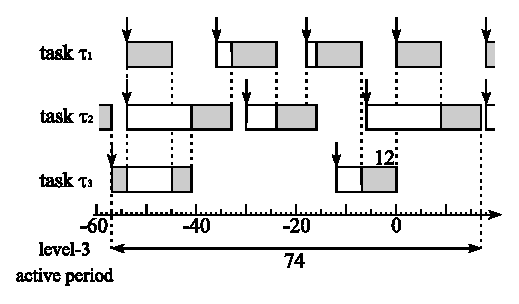
\includegraphics[width=.53\linewidth]{figures/example_1}
	\caption{A timeline for $\mathpzc{T}_{\ref{tab:ts_const_deadlines}}$ depicting a level-3 active period. The best-case response time of $\tau_3$ is assumed by the last job in the level-3 active period.}
	\label{fig:example_1}
\end{figure}


Figure \ref{fig:example_1} shows a timeline for task-set $\mathpzc{T}_{\ref{tab:ts_const_deadlines}}$ where the best-case response time of task $\tau_3$ is assumed by the last job in the level-3 active period. As can be seen, such a job cannot immediately start upon activation. On the other hand, when ignoring task $\tau_2$ from task-set $\mathpzc{T}_{\ref{tab:ts_const_deadlines}}$, the best-case response time of task $\tau_3$ is reduced to $\br^{\prime}_3 = 7$. Based on this observation, we conclude that, in general, the best-case response time of a task $\tau_i$ is not independent of the higher priority tasks that cannot preempt $\tau_i$. Therefore, we formulate the following fact.

\begin{fact} \label{fct:delaying_tasks}
	In FPTS, the best-case response time of a task $\tau_i$ can also be affected by a higher priority task that cannot preempt $\tau_i$, i.e. by delaying tasks in $\mathpzc{D_i}=\{\tau_d \in \mathpzc{T}|\theta_i \geq \pi_d > \pi_i\}$.
\end{fact}


Based on the optimal instant for FPPS, one may think that the best-case response time of a task $\tau_i$ under FPTS is found when the simultaneous activation of all high priority tasks that can preempt $\tau_i$ coincides with the completion of a job of $\tau_i$. Figure \ref{fig:example_1} seems to suggest that this is the case because an activation of $\tau_1$ coincides with the completion of the job of $\tau_3$ that assumes the best-case response time at time $t=0$. However, we now introduce an example that refutes this initial intuition.

\begin{table}[h]
	\center
	\caption{Task characteristics of $\mathpzc{T}_{\ref{tab:taskset_example2}}$.}
	\label{tab:taskset_example2}
	\begin{tabular}{c | c c c c c | c c c}
		\hline 
		task & $T_i$ & $\wcd_i$ & $C_i$ & $\pi_i$ & $\theta_i$ & $w\ell_i$ & $\wr_i$ & $\br_i$\\ 
		\hline 
		$\tau_1$& 35 & 20 & 5  & 4 & 4 & 1 &5 & 5\\ 
		$\tau_2$& 35 & 20 & 5  & 3 & 3 & 1 &10 & 5\\
		$\tau_3$& 50 & 65 & 20 & 2 & 2 & 2 &62 & 20\\ 
		$\tau_4$& 70 & 70 & 22 & 1 & 2 & 5 &66 & 27\\
		\hline 
	\end{tabular}
	\small
	\item The hyperperiod is $P^{\mathpzc{T}_{\ref{tab:taskset_example2}}}=350$ and $U^{\mathpzc{T}_{\ref{tab:taskset_example2}}}=1$.
\end{table}

Consider the set $\mathpzc{T}_{\ref{tab:taskset_example2}}$ of four tasks with characteristics as described in Table \ref{tab:taskset_example2}. Similarly to previous example, the values for the best-case response times were found using brute force. Furthermore, note that tasks $\tau_1$ and $\tau_2$ can preempt $\tau_4$. On the other hand, $\tau_3$ cannot preempt $\tau_4$ because $\pi_3 = \theta_4$. In order to investigate whether the best-case response time of $\tau_4$ can be found when all higher priority preemptive tasks are activated simultaneously, we repeated the simulation using brute force but now fixing the phasings of $\tau_1$ and $\tau_2$ to be always equal, i.e. $\varphi_1 = \varphi_2$. After performing the experiment, we found that the shortest response time of $\tau_4$ under these conditions is $BR^{\prime}_4 = 32$. Figure \ref{fig:example_2} depicts a timeline where this response time is found for the first job of $\tau_4$ in the level-4 active period. As can be seen, a simultaneous activation of tasks $\tau_1$ and $\tau_2$ coincides with the completion of a job of $\tau_4$ at time $t=0$. However, the best-case response time $BR_4=27$ is not assumed by any of the jobs of $\tau_4$ in the level-$4$ active period. Figure \ref{fig:example_3} shows a timeline for the same task-set $\mathpzc{T}_{\ref{tab:taskset_example2}}$ where the best-case response time of $\tau_4$ is assumed by its first job. Note that the activation of the preempting task $\tau_2$ does not coincide with the finalization time of the first job of $\tau_4$ where the best-case response time is found. Therefore, we propose the following fact as a first witness of dissimilarity between the best-case response time behavior of FPTS and FPPS.

\begin{fact}\label{fct:realese_preempt_tasks}
	In FPTS, the best-case response time of a task $\tau_i$ is not necessarily found when the simultaneous activation of all higher priority tasks that can preempt task $\tau_i$ coincides with the completion of one of its jobs.
\end{fact}

\begin{figure}[h]
	\centering
	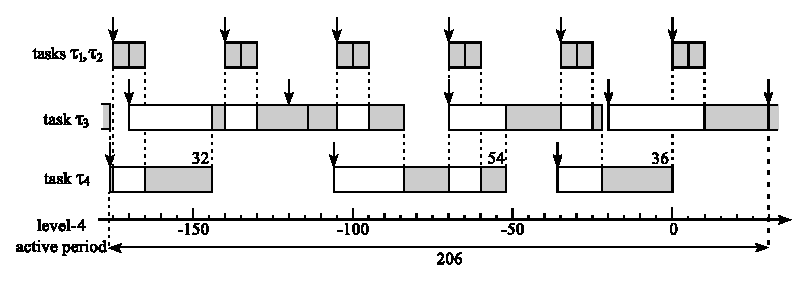
\includegraphics[width=.84\linewidth]{figures/example_2}
	\caption{A timeline for $\mathpzc{T}_{\ref{tab:taskset_example2}}$ depicting a level-4 active period. A simultaneous activation of preemptive tasks $\tau_1$ and $\tau_2$ coincides with a completion of the last job of $\tau_4$ in the level-4 active period at time $t=0$.}
	\label{fig:example_2}
\end{figure}


\begin{figure}[h]
	\centering
	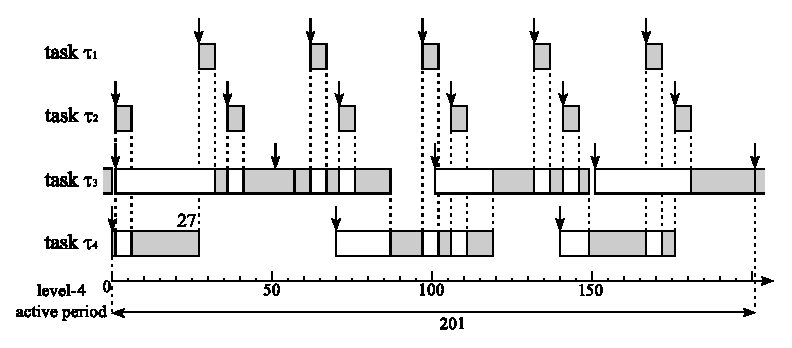
\includegraphics[width=.84\linewidth]{figures/example_3}
	\caption{A timeline for $\mathpzc{T}_{\ref{tab:taskset_example2}}$ depicting a level-4 active period where the best-case response time of task $\tau_4$ is assumed by the first job.}
	\label{fig:example_3}
\end{figure}

From Figure \ref{fig:example_3}, it is also interesting that, even that the first job of $\tau_4$ experiences a preemption by task $\tau_2$, it still assumes the best-case response time. On the other hand, the last job of $\tau_4$ in Figure \ref{fig:example_2} ending at time $t=0$ assumes the shortest hold time but not the best-case response time. This differs from the best-case behavior of FPPS, where the best-case response time is always assumed by the job with the shortest hold time. Hence, this is a second witness of dissimilarity.

\begin{fact} \label{cor:shortest_hold_time}The best-case response time under FPTS is not necessarily assumed by the job of $\tau_i$ with the shortest hold time.
\end{fact}



An important property in the best-case analysis for FPPS and arbitrary deadlines is that the best-case response time of a task $\tau_i$ is always assumed by the last job in a level-$i$ active period. However, this property does not hold for FPTS as can be seen in Figure \ref{fig:example_3} where the first job in a level-$4$ active period assumes the best-case response time. We have therefore found a third witness of dissimilarity.

\begin{fact}\label{fct:active_period}
	In FPTS, the best-case response time of a task $\tau_i$ is not necessarily assumed by the last job in a level-$i$ active period.
\end{fact}
\fi

\subsection{Tasks influencing the best-case response time}


According to Theorem \ref{thm:lower_prio_tasks}, lower priority tasks have no influence on the best-case response time of a task $\tau_i$. Therefore, we ignore lower priority tasks in the rest of this document. In addition, we distinguish between two types of tasks that can influence the {best-case response time} of a task $\tau_i$. These types of tasks are the set $\mathpzc{P_i}$ of \textit{preempting} tasks in $\{\tau_p \in \mathpzc{T} | \pi_p>\theta_i\}$, and the set $\mathpzc{D_i}$ of \textit{delaying} tasks given by Fact \ref{fct:delaying_tasks}. We termed the latter type as {delaying} tasks because they cannot preempt $\tau_i$ but at most can delay its start time. Furthermore, Fact \ref{cor:shortest_hold_time} shows that a job $\iota_{i,k^{\rm{br}}}$ of task $\tau_i$ that assumes the best-case response time does not necessarily have the shortest hold time. Instead, some preempting tasks may give rise to more preemptions in $\iota_{i,k^{\rm{br}}}$. Note that this is the case for the first job of $\tau_4$ starting at time $t=0$ in Figure \ref{fig:example_3}. This job assumes the best-case response time; however, it experiences a preemption from $\tau_2$. Based on this observation, we divide the set $\mathpzc{P_i}$ of preempting tasks of $\tau_i$  into the set of preempting tasks that give rise to \textit{extra preemptions} denoted as $\mathpzc{E_i} \subseteq \mathpzc{P_i}$, and the remaining preempting tasks that we call \textit{minimal preempting} tasks in the set $\mathpzc{M_i}=\mathpzc{P_i}\backslash\mathpzc{E_i}$.

\subsection{Properties for an optimal instant}

We now formulate some properties for an optimal instant for FPTS based on the tasks influencing the best-case response time of a task $\tau_i$.

\begin{theorem} \label{thm:optimal_instant_fpts}
	In FPTS, an optimal instant for a task $\tau_i$, where the best-case response time $\br_i$ is assumed by a job $\iota_{i,k^{\rm{br}}}$, has the following properties:
	\begin{itemize}
		\item \textbf{Activation of higher priority tasks.}
		An optimal instant occurs when the completion of $\iota_{i,k^{\rm{br}}}$ coincides with a simultaneous activation of all its {minimal preempting} tasks in $\mathpzc{M_i}$. Furthermore, the activation of all delaying tasks in $\mathpzc{D_i}$ and all {extra preempting} tasks in $\mathpzc{E_i}$ coincides with $s_{i,k^{\rm{br}}}+\Delta$, where $\Delta$ is a sufficiently small amount of time. 
		
		\item \textbf{Activation delays for minimal preempting and delaying tasks.}
		All minimal	preempting and delaying tasks experience a maximal activation delay at their respective simultaneous activation, and a minimal activation delay at previous activations.
		
		\item \textbf{Activation delays for extra preempting tasks.}
		Given that an extra preempting task $\tau_e$ preempts $\eta_e$ times to job $\iota_{i,k^{\rm{br}}}$, task $\tau_e$ experiences a maximal activation delay in the range $[0,\aj_e]$ at the moment of its simultaneous activation preserving the number of preemptions $\eta_e$. Furthermore, activations before $s_{i,k^{\rm{br}}}$ and in the interval $(s_{i,k^{\rm{br}}}+\Delta, f_{i,k^{\rm{br}}})$ experience a minimal activation delay.
	\end{itemize}

\end{theorem}



\begin{proof}
	\iffalse
	Let $k^{\rm{br}}$ be the job of a task $\tau_i$ that assumes its best-case response time, i.e. $R_{i,k^{\rm{br}}} = BR_i$. Furthermore, let $\Delta \in \mathbb{R^+}$ be a sufficiently small amount of time such that all jobs of higher priority tasks in $\mathpzc{P_i} \cup \mathpzc{D_i}$ activated after $s_{i,k^{\rm{br}}}$ are activated after $s_{i,k^{\rm{br}}}+\Delta$ as well. Figure \ref{fig:optimal_instant_proof_1} shows an example of a job of $\tau_i$ that assumes its best-case response time for task-set $\mathpzc{T}_{\ref{tab:ex_opt_instant_proof}}$. We will now show that it is always possible to construct an instant with the property given in Theorem \ref{thm:optimal_instant_fpts} for such a job $\iota_{i,k^{\rm{br}}}$ without increasing its response time. To this end, first recall that $R_{i,k^{\rm{\rm{br}}}} = S_{i,k^{\rm{br}}} + H_{i,k^{\rm{br}}}$; hence, we will show that the start time and the hold time of $k^{\rm{br}}$ do not increase when constructing such an instant with the property for an optimal instant.
	
	
	\begin{table}[h]
		\center
		\caption{Characteristics of task-set $\mathpzc{T}_{\ref{tab:ex_opt_instant_proof}}$.}
		\label{tab:ex_opt_instant_proof}
		\begin{tabular}{c | c c c c | c}
			\hline 
			task & $T_i$ & $C_i$ & $\pi_i$ & $\theta_i$ & $BR_i$\\ 
			\hline 
			$\tau_{p_1}$& 40 & 8  & 4 & 4 & 8\\ 
			$\tau_{p_2}$& 40 & 7  & 3 & 3 & 7\\ 
			$\tau_d$& 60 & 12 & 2 & 2 & 12\\ 
			$\tau_i$& 50 & 20 & 1 & 2 & 27\\
			\hline 
		\end{tabular}
		\small
		\item The hyperperiod is $P^{\mathpzc{T}_{\ref{tab:ex_opt_instant_proof}}}=600$ and $U^{\mathpzc{T}_{\ref{tab:ex_opt_instant_proof}}}=0.975$.
	\end{table}
	
	\begin{figure}[h]
		\centering
		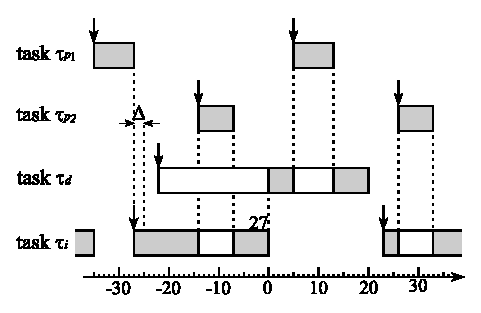
\includegraphics[width=0.45\linewidth]{figures/optimal_instant_proof_1_new} 
		\caption{A timeline for $\mathpzc{T}_{\ref{tab:ex_opt_instant_proof}}$ showing a job $k^{\rm{br}}$ of $\tau_i$ that assumes the best-case response time. All activations of higher priority tasks after $s_{i,k^{\rm{br}}}$ occur after $s_{i,k^{\rm{br}}} + \Delta$ as well.}
		\label{fig:optimal_instant_proof_1}
	\end{figure}
	
	\iffalse
	
	\begin{figure}[h]
		\centering
		\begin{tabular}{lll}
			a) Best-case response time for a job of $\tau_i$.&  & b) Adjusting delaying tasks. \\
			\includegraphics[width=0.45\linewidth]{figures/optimal_instant_proof_1} & &
			\includegraphics[width=0.45\linewidth]{figures/optimal_instant_proof_2} \\&& \\
			c) Adjusting best preemptive tasks. &  & d) Adjusting extra preemptive tasks.\\
			\includegraphics[width=0.45\linewidth]{figures/optimal_instant_proof_3} & &
			\includegraphics[width=0.45\linewidth]{figures/optimal_instant_proof_4} \\ 
		\end{tabular}
		
		\caption{Four timelines for task-set $\mathpzc{T}_{\ref{tab:ex_opt_instant_proof}}$ where the best-case response time $BR_i=27$ is assumed for the job of $\tau_i$. In a), all activations of higher priority tasks after $s_{i,k^{\rm{br}}}$ occur after $s_{i,k^{\rm{br}}} + \Delta$ as well. Furthermore, b) depicts the case where the delaying task $\tau_d$ is pushed till one activation coincides with $s_{i,k^{\rm{br}}} + \Delta$. In c), the preemptive task $\tau_{h_1}$ is pushed till one activation coincides with $f_{i,k^{\rm{br}}}$. Finally, d) shows the case where the preemptive task $\tau_{h_2}$ is pushed till one activation coincides with $s_{i,k^{\rm{br}}}+\Delta$. For this latter case, the optimal instant is obtained when $\mathpzc{P_i} = \{\tau_{h_1}\}$, $\mathpzc{E_i} = \{\tau_{h_2}\}$ and $\mathpzc{D_i} = \{\tau_{d}\}$.}
		\label{fig:optimal_instant_proof_1}
	\end{figure}
	\fi
	
	Let $k_d$ be the first job of a delaying task $\tau_d$ activated after $s_{i,k^{\rm{br}}}+\Delta$; hence, it holds that $a_{d,k_d} > s_{i,k^{\rm{br}}}+\Delta$. Furthermore, note that the pending load $P_{i-1}(s_{i,k^{\rm{br}}})$ of higher priority tasks at time $s_{i,k^{\rm{br}}}$ is zero; otherwise, job $\iota_{i,k^{\rm{br}}}$ would not be able to start at that moment. Clearly, if we push the activations of $\tau_d$ to an earlier moment in time till $a_{d,k_d} = s_{i,k^{\rm{br}}}+\Delta$, the pending load $P_{i-1}(s_{i,k^{\rm{br}}})$ remains zero. Hence, the start time cannot increase because job $\iota_{i,k^{\rm{br}}}$ can still start at the same time. Note that $\iota_{i,k^{\rm{br}}}$ cannot start earlier because this would reduce its response time, which is impossible because it assumes the best-case response time. In addition, the hold time cannot increase either because delaying tasks cannot preempt $\iota_{i,k^{\rm{br}}}$. We therefore conclude that changing the phasing of all delaying tasks in such a way that one of its activations occur at time $s_{i,k^{\rm{br}}}+\Delta$ does not change the response time of $\iota_{i,k^{\rm{br}}}$.  Figure \ref{fig:optimal_instant_proof_2} depicts this situation. As can be seen, the response time of the job of $\tau_i$ is preserved after pushing task $\tau_d$ till one of its activations occurs at time $s_{i,k^{\rm{br}}}+\Delta$.
	
	\begin{figure}[h]
		\centering
		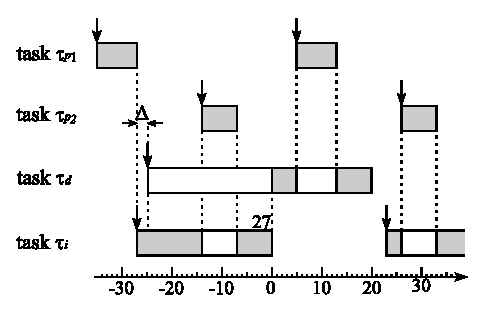
\includegraphics[width=0.45\linewidth]{figures/optimal_instant_proof_2_new} 
		\caption{A timeline for $\mathpzc{T}_{\ref{tab:ex_opt_instant_proof}}$ depicts the case when the delaying task $\tau_d$ is pushed till one activation coincides with $s_{i,k^{\rm{br}}} + \Delta$.}
		\label{fig:optimal_instant_proof_2}
	\end{figure}	
	
	Similarly, we will now show that it is always possible to modify the phasing of all preempting tasks till one of its activations occurs at time $s_{i,k^{\rm{br}}}+\Delta$ or at time $f_{i,k^{\rm{br}}}$ without affecting the response time. To this end, let $k_e$ be the first job activated after $s_{i,k^{\rm{br}}}+\Delta$ of a preempting task $\tau_p$; hence, $a_{p,k_e} > s_{i,k^{\rm{br}}}+\Delta$. In addition, let $k_m$ be the first job of $\tau_p$ activated at or after time $f_{i,k^{\rm{br}}}$; hence, $a_{p,k_m} \geq f_{i,k^{\rm{br}}}$. We now divide the proof in two cases.
	
	\{\textit{Case} $a_{p,k_e}-(s_{i,k^{\rm{br}}} + \Delta) > a_{p,k_m}-f_{i,k^{\rm{br}}}$\} For this case, note that it is possible to push the activations of $\tau_p$ to an earlier moment in time till $a_{p,k_m}=f_{i,k^{\rm{br}}}$. After doing so, it still holds that $a_{p,k_e} > s_{i,k^{\rm{br}}}+\Delta$. Therefore, $\iota_{i,k^{\rm{br}}}$ still experiences the same number of preemptions by $\tau_p$ and its hold time $H_{i,k^{\rm{br}}}$ remains unchanged. Furthermore, similarly to the case for delaying tasks, $\iota_{i,k^{\rm{br}}}$ can still start at the same time because the pending load $P_{i-1}(s_{i,k^{\rm{br}}})$ remains zero. Therefore, the start time $S_{i,k^{\rm{br}}}$ do not increase either. Figure \ref{fig:optimal_instant_proof_3} shows that indeed the response time of the job of $\tau_i$ remains the same after pushing task $\tau_{h_1}$.
	
	\begin{figure}[h]
		\centering
		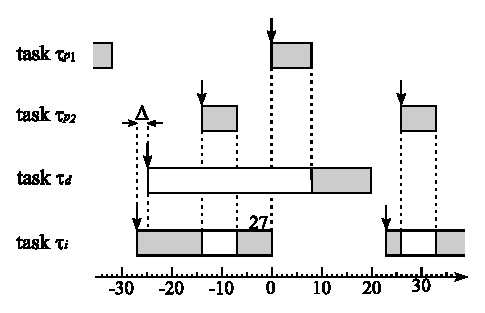
\includegraphics[width=0.45\linewidth]{figures/optimal_instant_proof_3_new} 
		\caption{A timeline for $\mathpzc{T}_{\ref{tab:ex_opt_instant_proof}}$ depicts the case when the delaying task $\tau_d$ is pushed till one activation coincides with $s_{i,k^{\rm{br}}} + \Delta$.}
		\label{fig:optimal_instant_proof_3}
	\end{figure}
	
	\{\textit{Case} $a_{p,k_e}-(s_{i,k^{\rm{br}}} + \Delta) \leq a_{p,k_m}-f_{i,k^{\rm{br}}}$\} Similar to previous case, we push the activations of $\tau_p$ earlier in time till $a_{p,k_e} = s_{i,k^{\rm{br}}}+\Delta$. Note that it still holds that $a_{p,k_m} \geq f_{i,k^{\rm{br}}}$. Hence, the hold time $H_{i,k^{\rm{br}}}$ will remain unchanged because $\iota_{i,k^{\rm{br}}}$ still experiences the same number of preemptions. Furthermore, since it still holds that $a_{p,k_e} > s_{i,k^{\rm{br}}}$, job $\iota_{i,k^{\rm{br}}}$ can still start at the same time because there is no pending load of higher priority tasks at that time. Figure \ref{fig:optimal_instant_proof_4} shows that, after pushing the activations of $\tau_{h_2}$, the response time of the job of $\tau_i$ is preserved.
	
	We conclude that the phasing of all preempting tasks can be changed in such a way that, for each of its tasks, one of its activations occurs at time $s_{i,k^{\rm{br}}} + \Delta$ or at time $ f_{i,k^{\rm{br}}} $ without affecting the response time $R_{i,k^{\rm{br}}}$.
	\fi
\end{proof}

\iffalse
\begin{figure}[h]
	\centering
	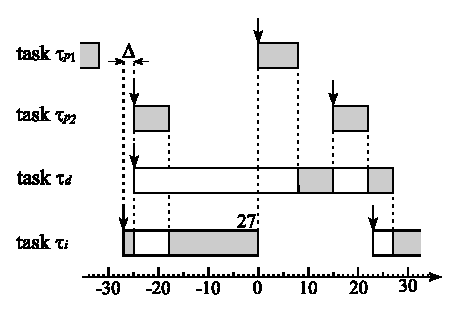
\includegraphics[width=0.45\linewidth]{figures/optimal_instant_proof_4_new} 
	\caption{Add caption}
	%\caption{A timeline for $\mathpzc{T}_{\ref{tab:ex_opt_instant_proof}}$ depicts the case when the delaying task $\tau_d$ is pushed till one activation coincides with $s_{i,k^{\rm{br}}} + \Delta$.}
	\label{fig:optimal_instant_proof_4}
\end{figure}
\fi

Note that, given a task-set $\mathpzc{T}$ and a task $\tau_i \in \mathpzc{T}$, the set of {delaying} tasks $\mathpzc{D_i}$ is empty when the preemption threshold of $\tau_i$ is equal to its priority. Furthermore, the set of extra preempting tasks $\mathpzc{E_i}$ is always empty when there are no delaying tasks. Therefore, we conclude that the properties of an optimal instant for a task $\tau_i$ scheduled under FPTS described in Theorem \ref{thm:optimal_instant_fpts} gives rise to an optimal instant for FPPS when $\theta_i = \pi_i$. 

Figure \ref{fig:optimal_instant_proof_4}\footnote{PENDING TO ADD FIGURE} shows an example of these properties for an optimal instant under FPTS for task $\tau_i$. As can be seen, the activation of the minimal preempting task $\tau_{p_1}$ coincides with the completion of the job of task $\tau_i$ at time $t=0$. Furthermore, {delaying} task $\tau_d$ and extra preempting task $\tau_{p_2}$ are activated an instant $\Delta$ after the start of $\tau_i$.

It is worth noting that, from the properties for an optimal instant given above, it is not clear how to partition the set of preempting tasks $\mathpzc{P_i}$ into the (sub-)sets of extra preempting $\mathpzc{E_i}$ and minimal preempting $\mathpzc{M_i}$ tasks. In fact, we could have chosen $\mathpzc{E_i}=\{\tau_{p_1}\}$ and $\mathpzc{M_i}=\{\tau_{p_2}\}$ in the example depicted in Figure \ref{fig:optimal_instant_proof_4}, and we would still have obtained an option that is in accordance with the properties described in Theorem \ref{thm:optimal_instant_fpts}. However, this new option does not lead to the best-case response time. Therefore, we conclude that in FPTS there may be multiple candidates of optimal instants that we have to explore in order to find the best-case response time of a task $\tau_i$. Clearly, this differs from the best-case analysis for FPPS, where the way to construct an optimal instant is always unique. Given this observation, our best-case analysis is based on exploring all possible partitions of preempting tasks into the sets of extra preempting and minimal preempting tasks.

\iffalse
\subsection{The phasing of delaying and extra preempting tasks} \label{sec:phasing_delaying_extra}

According to Theorem \ref{thm:optimal_instant_fpts}, the simultaneous activation of minimal preempting tasks has to take place at time $t_1=f_{i,k^{\rm{opt}}}$, where $\iota_{i,k^{\rm{opt}}}$ is the job of $\tau_i$ experiencing the properties for an optimal instant. Furthermore, the simultaneous activation of delaying and extra preempting tasks occurs at time $t_2=s_{i,k^{\rm{opt}}}+\Delta$. In this section, we aim to determine the phasing at which delaying and extra preempting tasks must be simultaneously activated relative to the activation of minimal preempting tasks (i.e. relative to $t_1$).


Therefore, the activation time $a_r$ for delaying and extra preempting tasks relative to the activation of minimal preempting tasks is given by
\begin{align} \label{eqn:relative_activation_extra_delaying}
a_r = t_2 - t_1 = (s_{i,k^{\rm{opt}}}+\Delta) - f_{i,k^{\rm{opt}}} = -H_{i,k^{\rm{opt}}}+\Delta.
\end{align}

Note that the hold time of job $k^{\rm{br}}$ is needed to determine the relative activation of delaying and extra preempting tasks. We therefore derive the following corollary.
\begin{corollary} \label{cor:hold_time_dor_optimal_instant}
	In order to construct an instant with the property given by Theorem \ref{thm:optimal_instant_fpts}, it is necessary to first determine the hold time $H_{i,k^{\rm{br}}}$ of the job that assumes the best-case response time.
\end{corollary}

\fi

\subsection{The activation delay of higher priority tasks}

Recall from Theorem \ref{thm:optimal_instant_fpts} that the activation delay $\alpha_j$ of a minimal preempting or a delaying task $\tau_j$ is maximal at the moment of its simultaneous activation; hence, it holds that
\begin{align}\label{eqn:activation_delay_minimal_delaying}
	\alpha_j = \aj_j \hspace{.6cm} \textnormal{for all $\tau_j \in \mathpzc{M}_i \cup \mathpzc{D}_i$}.
\end{align}
Furthermore, the maximal activation delay of an extra preempting task $\tau_e$ at the moment of its simultaneous activation is constrained by the number of times $\eta_e$ that preempts to the job with a best-case response time; moreover, this activation delay is in the range $[0,\aj_e]$. Therefore, it is necessary to first determine the number of preemptions for each of the extra preempting tasks to derive their activation delays. To this end, we first introduce the notion of \textit{preemption vector} as follows.

\begin{definition}
	\textit{Preemption vector}.
	Let $\iota_{i,k^{\rm{opt}}}$ be a job of $\tau_i$ that experiences the properties for an optimal instant as described in Theorem \ref{thm:optimal_instant_fpts}. A preemption vector $\vec{\eta}$ of $\iota_{i,k^{\rm{opt}}}$ is a $|\mathpzc{P}_i|$-dimensional vector such that $\vec{\eta}=(\eta_1, \eta_2,\dots,\eta_{|\mathpzc{P}_i|})$ where $\eta_p$ corresponds to the number of times that a preempting task $\tau_p$ preempts to $\iota_{i,k^{\rm{opt}}}$.
\end{definition}

Based on a preemption vector, the calculation of the hold time of a job experiencing the properties for an optimal instant is straightforward.

\begin{corollary}
Let $\iota_{i,k^{\rm{opt}}}$ be a job of $\tau_i$ that experiences the properties for an optimal instant and let $\vec{\eta}$ be its corresponding preemption vector. The hold time $h_i(\vec{\eta})$ of $\iota_{i,k^{\rm{opt}}}$ is given by
\begin{align}
	h_i(\vec{\eta})= \bc_i + \sum\limits_{p:\tau_p \in \mathpzc{P}_i} \eta_p \cdot \bc_p.
\end{align}
\end{corollary}


Figure \ref{fig:alpha_e} shows and example of the activation delay $\alpha_e$ for an arbitrary extra preempting task $\tau_e$. Note that the first job of $\tau_e$ is activated in the middle of its activation interval at a time $t=s_{i,k^{\rm{opt}}}+\Delta$ resulting in $\alpha_e < \aj_e$. Furthermore, note that $\alpha_e$ cannot increase because $\eta_e = 3$. Increasing $\alpha_e$ would result in an additional preemption by the last job of $\tau_e$ in job $\iota_{i,k^{\rm{opt}}}$; hence, violating the constraint of $\eta_e = 3$. We now derive a corollary to determine the maximal activation delay of extra preempting tasks as follow.

\begin{figure}[h]
	\centering
	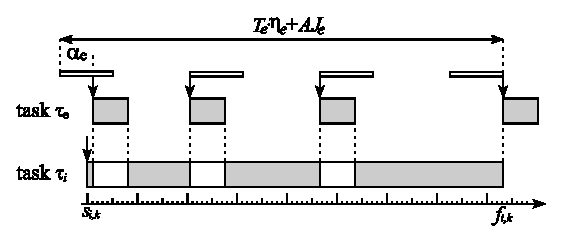
\includegraphics[width=0.7\linewidth]{figures/alpha_e} 
	\caption{An example where the activation delay $\alpha_e$ of an extra preempting task $\tau_e$ is constrained by the number of times $\eta_e = 3$ that it preempts to job $\iota_{i,k^{\rm{opt}}}$ as described in Theorem \ref{thm:optimal_instant_fpts}. Furthermore, note that the activation delay of the jobs of $\tau_e$ during interval $(s_{i,k^{\rm{opt}}} + \Delta,f_{i,k^{\rm{opt}}})$ is minimal.}
	\label{fig:alpha_e}
\end{figure}


\begin{corollary}\label{cor:activation_delay_formula}
	Let $\iota_{i,k^{\rm{opt}}}$ be a job of $\tau_i$ that experiences the properties for an optimal instant and let $\vec{\eta}$ be its corresponding preemption vector. Furthermore, let $\tau_e$ be an extra preempting task of such a job. The maximal activation delay $\alpha_e(\vec{\eta},\Delta)$ of the job of $\tau_e$ activated at time $t = s_{i,k^{\rm{opt}}}+\Delta$ is given by
	\begin{align} \label{eqn:activation_delay_formula}
		\alpha_e(\vec{\eta},\Delta) = \min(T_e \cdot \eta_e + \aj_e + \Delta - h_i(\vec{\eta}), \aj_e)^+ \hspace{.6cm} \textnormal{for all $\tau_e \in \mathpzc{E}_i$}.
	\end{align}
\end{corollary}

The outer $\min$ and superscript $(+)$ operator in Equation (\ref{eqn:activation_delay_formula}) keep $\alpha_e(\vec{\eta},\Delta)$ within the range $[0,\aj_e]$. Furthermore, the term $T_e \cdot \eta_e + \aj_e$ is the time length from the start of the activation interval of the job of $\tau_e$ activated just after $\iota_{i,k^{\rm{opt}}}$ starts and the end of the activation interval of the first job of $\tau_e$ that is activated at $t \geq f_{i,k^{\rm{opt}}}$. Figure \ref{fig:alpha_e} depicts this situation. Combining Equations (\ref{eqn:activation_delay_minimal_delaying}) and (\ref{eqn:activation_delay_formula}), we derive a more general formula for the activation delay of higher priority tasks as follows.
\begin{align} \label{eqn:activation_delay}
	\alpha_j(\vec{\eta},\Delta) = \begin{cases} 
	\min(T_j \cdot \eta_j + \aj_j + \Delta - h_i(\vec{\eta}), \aj_j)^+ & \text{for all} \hspace{3mm} \tau_j \in \mathpzc{E}_i\\
	\aj_j & \text{for all} \hspace{3mm} \tau_j \in \mathpzc{M}_i \cup \mathpzc{D}_i
	\end{cases}
\end{align}


\section{Determining the preemption vectors of a job}\label{sec:hold_times_of_a_job}
\iffalse
From Corollary \ref{cor:activation_delay_formula}, we have to determine first the preemption vector of a job that assumes the best-case response time in order to determine the activation delays of its extra preempting tasks and subsequently construct an optimal instant. Note that this job does not necessarily has a preemption vector that leads to the shortest hold time (Fact \ref{cor:shortest_hold_time}). Hence, we propose to explore all possible preemption vectors of a job experiencing an optimal instant in order to determine the one that leads to the best-case response time.

In this section, we first show how to determine the maximum and minimum possible preemption vectors of a job given a set of extra preempting tasks. In case these vectors result to be different, we compute the preemption vectors falling in between.

\subsection{Maximum and minimum preemption vectors}
First, note that the hold time of a job is only influenced by the amount of preemptions that it experiences by its extra and minimal preempting tasks. Therefore, we derive all the possible hold times given a set of extra preempting tasks. To this end, we first introduce the notions of maximal, minimal and best-case hold intervals.

%\begin{definition}
%	The \textit{maximal hold interval} $\wh^{\rm{max}}_i(y,\mathpzc{E})$ is defined as the worst-case hold time of an artificial task $\tau^{\prime}_i$ with a computation time of $y \in \mathbb{R}^+$ in the task-set $\mathpzc{E}\cup \{\tau^{\prime}_i\}$ given that all jobs in the interval assume their {best-case computation times}.
%\end{definition}

\begin{definition}
The \textit{maximal hold interval} $\hi^{\rm{ma}}_i(y,\mathpzc{E})$ and the \textit{minimal hold interval} $\hi^{\rm{mi}}_i(y,\mathpzc{E})$ are defined as the maximal and minimal hold times of a job $\iota_{i,k}$ of an artificial task $\tau^{\prime}_i$ with a computation time $y \in \mathbb{R}^+$ when such a job $\iota_{i,k}$ experiences extra preemptions by the tasks in $\mathpzc{E}$, i.e. the tasks in  $\mathpzc{E}$ are activated just after job $\iota_{i,k}$ starts. In addition, all jobs in the interval assume their best-case computation times.
\end{definition}

The {maximal hold interval} $\hi^{\rm{ma}}_i(y,\mathpzc{E})$ follows directly from the formula for {worst-case hold time} for FPTS given in \cite{BAHDB17}. The only difference is that best-case computation times are assumed for the {maximal hold interval}. Hence, $\hi^{\rm{ma}}_i(y,\mathpzc{E})$ is given by the smallest $x \in \mathbb{R}^+$ satisfying
\begin{align}
x = y + \sum\limits_{e:\pi_e > \theta_i, \tau_e \in \mathpzc{E}}\Big\lceil  \dfrac{x+ \aj_e}{T_e}\Big\rceil  BC_e.
\end{align}

Similarly, the {minimal hold interval} $\hi^{\rm{mi}}_i(y,\mathpzc{E})$ is given by the smallest $x \in \mathbb{R}^+$ satisfying
\begin{align}
x = y + \sum\limits_{e:\pi_e > \theta_i, \tau_e \in \mathpzc{E}}\Big\lceil  \dfrac{x- \aj_e}{T_e}\Big\rceil^{*}  BC_e,
\end{align}
where the notation $w^*$ stands for $\max(w,1)$.

\begin{definition} \label{def:best_case_interval}
	The \textit{best-case hold interval} $\bh_i(y,\mathpzc{M})$ is defined as the best-case hold time of an artificial task $\tau^{\prime}_i$ with a computation time of $y \in \mathbb{R}^+$ in the task-set $\mathpzc{M}\cup \{\tau^{\prime}_i\}$ given that $\mathpzc{M}$ contains only preempting tasks.
\end{definition}

Since Definition \ref{def:best_case_interval} assumes that $\mathpzc{M}$ only contains preempting tasks, we can use the same formula for the best-case hold time for FPPS given in \cite{BFV08}\footnote{In \cite{BFV08}, the term best-case hold time is referred as best-case execution time.} to calculate $\bh_i(y,\mathpzc{M})$. Hence, function $\bh_i(y,\mathpzc{M})$ returns the largest positive solution of $x \in \mathbb{R}^+$ satisfying
\begin{align} \label{eqn:best_case_hold_interval}
x = y + \sum\limits_{m:\pi_m > \theta_i, \tau_m \in \mathpzc{M}} \Big( \Big\lceil  \dfrac{x-\aj_m}{T_m}\Big\rceil -1 \Big)^+  BC_m.
\end{align}


Finally, we introduce the set of hold times of a task $\tau_i$ based on its extra and minimal preempting tasks.

\begin{definition} \label{def:ht}
	The set of hold times $\hlt_i(\mathpzc{E}_i)$ is defined as the set of all possible hold times that a job $\iota_{i,k}$ of $\tau_i\in \mathpzc{T}$ can have when experiencing extra preemptions by the tasks in $\mathpzc{E}_i \subseteq \mathpzc{P_i}$ and minimal preemptions by the tasks in $\mathpzc{M}_i = \mathpzc{P_i} \backslash \mathpzc{E}_i$. This is, when the tasks in $\mathpzc{E}_i$ are simultaneously activated at time $s_{i,k}+\Delta$, where $\Delta$ is a sufficiently small amount of time to experience such extra preemptions.  Furthermore, delaying tasks of $\tau_i$ in $ \mathpzc{T}$ are ignored.
\end{definition}

Clearly, given a set of extra preempting tasks $\mathpzc{E}_i$, a hold time $h \in \hlt_i(\mathpzc{E}_i)$ is given by the following equation:
\begin{align} \label{eqn:hold_time}
h = \beta_M + \beta_E + BC_i,
\end{align}
where $\beta_M,\beta_E \in \mathbb{R^+} \cup \{0\}$ are the amount of time spent by preemptions of minimal preempting and extra preempting tasks in the hold time $h$ respectively. Furthermore, it is possible to determine the minimum possible values of $\beta_M$ and $\beta_E$ by solving the following set of recursive equations starting with a lower bound:
%
% Furthermore, the values of $\beta_m$ and $\beta_e$ are given by the following set of recursive equations:
\begin{flalign} \label{eqn:beta_e}
\begin{split}
\beta^{\rm{mi}}_E = \hi^{\rm{mi}}_i(\beta^{\rm{mi}}_M+ BC_i,\mathpzc{E}_i) - \beta^{\rm{mi}}_M - BC_i,\\
\beta^{\rm{mi}}_M = \bh_i(\beta^{\rm{mi}}_E + BC_i,\mathpzc{M}_i) - \beta^{\rm{mi}}_E- BC_i.% \label{eqn:beta_m}
\end{split}
\end{flalign}
Note that the first equation in (\ref{eqn:beta_e}) minimizes the influence of extra preempting tasks using the minimal hold interval $\hi^{\rm{mi}}_i(y,\mathpzc{E})$. On the other hand, the second equation minimizes the influence of minimal preempting tasks using the best-case hold interval  $\bh_i(y,\mathpzc{M})$. Similarly, the maximum possible values of $\beta_M$ and $\beta_E$ can be derived using the maximal hold interval $\hi^{\rm{ma}}_i(y,\mathpzc{E})$. More precisely, by solving the following set of recursive equations starting with an upper bound. This set of equations maximizes the influence of extra preempting tasks in the hold time.
\begin{flalign} \label{eqn:beta_max}
\begin{split}
\beta^{\rm{ma}}_E = \hi^{\rm{ma}}_i(\beta^{\rm{ma}}_M+ BC_i,\mathpzc{E}_i) - \beta^{\rm{ma}}_M - BC_i,\\
\beta^{\rm{ma}}_M = \bh_i(\beta^{\rm{ma}}_E + BC_i,\mathpzc{M}_i) - \beta^{\rm{ma}}_E- BC_i.% \label{eqn:beta_m}
\end{split}
\end{flalign}

Once the maximum and minimum values of $\beta_M$ and $\beta_E$ are determined using the sets of recursive equations in (\ref{eqn:beta_e}) and (\ref{eqn:beta_max}), the minimum ($h^{\rm{mi}}$) and the maximum ($h^{\rm{ma}}$) hold times of a job in the set $\mathpzc{H}_i(\mathpzc{E}_i)$ can be derived using Equation (\ref{eqn:hold_time}). In general, the set of hold times $\mathpzc{H}_i(\mathpzc{E}_i)$ may contain values in the range $[h^{\rm{mi}}, h^{\rm{ma}}]$. However, when $h^{\rm{ma}} = h^{\rm{mi}}$, then this is the only possible hold time for a job of $\tau_i$ that experiences extra preemptions by the tasks in $\mathpzc{E}_i$; hence, $\hlt_i(\mathpzc{E}_i)$ is a singleton for this case.

As an example where more than one hold time can be found, consider the set of tasks with characteristics as described in Table \ref{tab:ex_hold_times}. Let $\tau_1$ be an extra preempting task of $\tau_4$, and $\tau_2$ a minimal preempting task, i.e. $\mathpzc{E}_4=\{\tau_1\}$ and $\mathpzc{M}_4=\{\tau_2\}$. After solving the sets of recursive equations (\ref{eqn:beta_max}) and (\ref{eqn:beta_e}) for task $\tau_4$, we find that the maximum and minimum hold times of a job of $\tau_4$ are $h^{\rm{ma}}=24$ and $h^{\rm{mi}}=18$ respectively. Figure \ref{fig:max_min_hold_times} depicts two timelines in which these hold times are found for a job of task $\tau_4$. As can be seen, in both cases $\tau_1$ is activated just after the start time of the job of $\tau_4$; hence, $\tau_1$ is an extra preempting task. In addition, an activation of $\tau_2$ coincides with the completion of the job of $\tau_4$ also for both cases. Note that task $\tau_3$ is not considered because, being a delaying task, it cannot preempt $\tau_4$. 

\begin{table}[h]
	\center
	\caption{Characteristics of task-set $\mathpzc{T}_{\ref{tab:ex_hold_times}}$.}
	\label{tab:ex_hold_times}
	\begin{tabular}{c | c c c c c}
		\hline 
		task & $T_i$ & $C_i$ & $\aj_i$ & $\pi_i$ & $\theta_i$ \\% & $\br_i$\\%& $\br_i$\\% & $H^{\rm{min}}_i$\\ 
		\hline 
		$\tau_1$& 8  & 2  & 4 & 4 & 4 \\%& 10\\%& 10 % & 10 \\ 
		$\tau_2$& 10 & 2  & 1 & 3 & 3 \\%& 12\\%& 20 % & 20 \\ 
		$\tau_3$& 20 & 1  & 3 & 2 & 2 \\%& 8 \\%& 2  % & 2 \\ 
		$\tau_4$& 40 & 12 & 2 & 1 & 2 \\%& 36\\%& 60 % & 60 \\
		\hline 
	\end{tabular}
	\small
	\item The hyperperiod is $P^{\mathpzc{T}_{\ref{tab:ex_hold_times}}}=40$ and $U^{\mathpzc{T}_{\ref{tab:ex_hold_times}}} = 0.8$.
\end{table}

\begin{figure}[H]
	\centering
	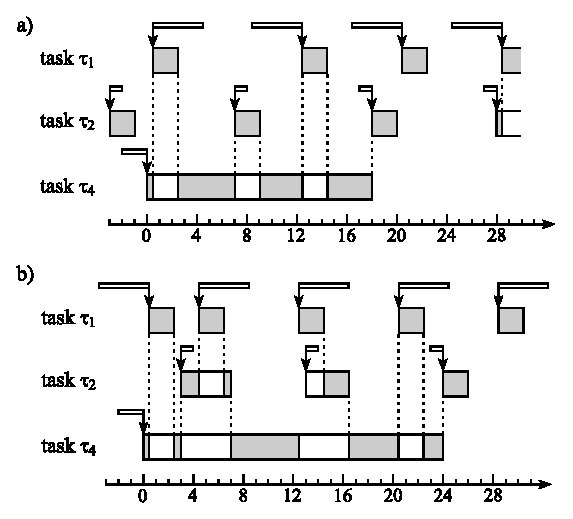
\includegraphics[width=0.7\linewidth]{figures/max_min_hold_times} 
	\caption{Two timelines for $\mathpzc{T}_{\ref{tab:ex_hold_times}}\backslash\{\tau_3\}$ showing the minimum (top) and maximum (bottom) hold times for a job of $\tau_4$ when experiencing extra preemptions by $\tau_1$ and minimal preemptions by $\tau_2$.}
	\label{fig:max_min_hold_times}
\end{figure}

\subsection{Intermediate hold times}

We propose to evaluate all intermediate hold times in the range $[h^{\rm{mi}}, h^{\rm{ma}}]$ to determine the remaining values in the set $\mathpzc{H}_i(\mathpzc{E}_i)$. It is possible to evaluate all intermediate values because the number of preemptions $\eta_p$ that a preempting task $\tau_p$ causes in a job of a task $\tau_i$ is integer and finite. Furthermore, this number of preemptions that a job of $\tau_i$ experiences is bounded as follows: 
\begin{align} \label{eqn:bound_np}
\begin{split}
\Big\lceil  \dfrac{h^{\rm{mi}} - \aj_e}{T_e}\Big\rceil^* \leq \eta_e \leq \Big\lceil  \dfrac{h^{\rm{ma}}+ \aj_e}{T_e}\Big\rceil \hspace{5mm} \text{for $\tau_e \in \mathpzc{E}_i$}, \\
\Big(\Big\lceil  \dfrac{h^{\rm{mi}} - \aj_m}{T_m}\Big\rceil-1\Big)^+ \leq \eta_m \leq \Big(\Big\lceil  \dfrac{h^{\rm{ma}} - \aj_m}{T_m}\Big\rceil - 1\Big)^+ \hspace{5mm} \text{for $\tau_m \in \mathpzc{M}_i$}
\end{split}
\end{align}

The process of finding intermediate hold times in the set $\mathpzc{H}_i(\mathpzc{E}_i)$ therefore starts by choosing a candidate number of preemption $\eta_p$ in the range given in (\ref{eqn:bound_np}) for each preempting task. Given these number of preemptions, the corresponding values for $\beta_E$ and $\beta_M$ can alternatively be derived as follows:
\begin{align} \label{eqn:beta_2}
\beta_E = \sum\limits_{e:\tau_e \in \mathpzc{E}_i} \eta_e \cdot BC_e, \text{\hspace{14mm}}
\beta_M = \sum\limits_{m:\tau_m \in \mathpzc{M}_i} \eta_m \cdot BC_m.
\end{align}
Afterwards, the candidate hold time $h^{\rm{ca}}\in[h^{\rm{mi}}, h^{\rm{ma}}]$ that we wish to evaluate is simply found using Equation (\ref{eqn:hold_time}). To find whether $h^{\rm{ca}}$ is a valid candidate, we first introduce the notion of \textit{hold interval}.

\begin{definition} \label{def:hold_interval}
	The \textit{hold interval} $\hi_i(y,\mathpzc{E}_i)$ is defined as the hold time of a job $\iota_{i,k}$ of an artificial task $\tau^{\prime}_i$ with a computation time $y \in \mathbb{R}^+$ when such a job $\iota_{i,k}$ experiences extra preemptions by the tasks in $\mathpzc{E}_i$ according to the properties of optimal instant described in Theorem \ref{thm:optimal_instant_fpts}. In addition, all jobs in the interval assume their best-case computation times.
\end{definition}

The hold interval $\hi_i(y,\mathpzc{E}_i)$ is given by the smallest $x \in \mathbb{R}^+$ satisfying the following recursive equation:
\begin{align} \label{eqn:hold_interval}
x = y + \sum\limits_{e:\tau_e \in \mathpzc{E_i}}\Big\lceil  \dfrac{x+ g_e(x)}{T_e}\Big\rceil^{*}  BC_e,
\end{align}
where function $g_e(x)$ is defined as follow:
\begin{align}
	g_e(x) = 
	\begin{cases} 
	\alpha_e & \text{if} \hspace{3mm} \Big\lceil \dfrac{x+ \alpha_e}{T_e} \Big\rceil \leq \eta_e \\
	\alpha_e - \aj_e & \text{otherwise.}
	\end{cases}
\end{align}
The activation delay $\alpha_e$ of an extra preempting task can be derived by Equation (\ref{eqn:alpha_e}) using the chosen number of preemptions $\eta_e$ and the candidate hold time $h^{\rm{ca}}$.

Recall that Equation (\ref{eqn:hold_interval}) can be solved by an iterative procedure starting with a lower bound. Moreover, the result of $\hi_i(y,\mathpzc{E}_i)$ increases in every iteration till we arrive to a fixed point. During this iterative procedure, function $g(x)$ returns $\alpha_e$ when there are $\eta_e$ or less jobs of task $\tau_e$ preempting the hold time given by the intermediate result of $\hi_i(y,\mathpzc{E}_i)$. Therefore, these jobs of $\tau_e$ have minimal activation delay as described by Theorem \ref{thm:optimal_instant_fpts}. Furthermore, for latter jobs of $\tau_e$, function $g(x)$ returns $\alpha_e - \aj_e$ which means that these jobs have a maximal activation delay.

In order to find whether $h^{\rm{ca}}$ is a valid candidate, the following equations must hold:
\begin{flalign} \label{eqn:test_h_cand}
\begin{split}
h^{\rm{ca}} = \hi_i(\beta_M+ BC_i,\mathpzc{E}_i),\\
h^{\rm{ca}} = \bh_i(\beta_E + BC_i,\mathpzc{M}_i).
\end{split}
\end{flalign}
If both equations in (\ref{eqn:test_h_cand}) hold, then $h^{\rm{ca}}$ is a valid hold time for a job of $\tau_i$ and it is contained in the set $\mathpzc{H}_i(\mathpzc{E}_i)$. We can repeat this process evaluating candidates of hold times until we have explored all possible number of preemptions of preempting tasks bounded by (\ref{eqn:bound_np}).

As an example, consider again the set of tasks $\mathpzc{T}_\ref{tab:ex_hold_times}$ described in Table \ref{tab:ex_hold_times}. Let $\tau_1$ be an extra preempting task and $\tau_2$ a minimal preempting task of $\tau_4$. Recall that the minimum and maximum hold times for a job of $\tau_4$ are $h^{\rm{mi}}=18$ and $h^{\rm{ma}}=24$ respectively (see Figure \ref{fig:max_min_hold_times}). Based on this and using the bounds in (\ref{eqn:bound_np}), the number of preemptions $\eta_1$ and $\eta_2$ that tasks $\tau_1$ and $\tau_2$ cause in a job of $\tau_4$ is bounded by $2 \leq \eta_1 \leq 4$ and $1 \leq \eta_2 \leq 2$. Table \ref{tab:ex_intermediate_hold_times} summarizes the result of the evaluation of the intermediate hold times considering the aforementioned bounds for $\eta_1$ and $\eta_2$. As can be seen, there are three hold times that satisfy the equations in (\ref{eqn:test_h_cand}). Those are the minimum and maximum hold times (trivial case) and an intermediate hold time $h=22$; therefore, $\hlt_4(\{\tau_1\}) = \{18,22,24\}$. Figure \ref{fig:intermediate_hold_time} shows a timeline in which such an intermediate hold time is assumed by a job of $\tau_4$.

\begin{table}[h]
	\center
	\caption{Evaluation of intermediate candidates of hold times for task $\tau_4 \in \mathpzc{T}_\ref{tab:ex_hold_times}$. A candidate hold time is considered valid when the set of equations in (\ref{eqn:test_h_cand}) hold.}
	\label{tab:ex_intermediate_hold_times}
	\begin{tabular}{c c | c c | c c c}
		\hline 
		$\eta_1$ & $\eta_2$ & $\beta_1$ & $\beta_2$ & $h^{\rm{ca}}$ & $\alpha_1$ & Valid\\
		\hline 
		2 & 1 & 4 & 2 & 18 & 2 & \cmark \\
		2 & 2 & 4 & 4 & 20 & 0 & \xmark \\ 
		3 & 1 & 6 & 2 & 20 & 4 & \xmark \\ 
		3 & 2 & 6 & 4 & 22 & 4 & \cmark \\
		4 & 1 & 8 & 2 & 22 & 4 & \xmark \\ 
		4 & 2 & 8 & 4 & 24 & 4 & \cmark \\
		\hline 
	\end{tabular}
\end{table}

\begin{figure}[h]
	\centering
	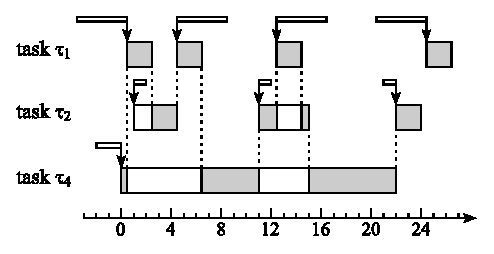
\includegraphics[width=0.62\linewidth]{figures/example_intermediate_hold_time} 
	\caption{A timeline for $\mathpzc{T}_{\ref{tab:ex_hold_times}}\backslash\{\tau_3\}$ showing the intermediate hold time assumed by a job of $\tau_4$ when experiencing extra preemptions by $\tau_1$ and minimal preemptions by $\tau_2$.}
	\label{fig:intermediate_hold_time}
\end{figure}

\fi
\iftrue
\section{Exact best-case response time analysis}
In this chapter, we present and prove a novel exact best-case response time analysis for independent real-time periodic tasks with arbitrary deadlines scheduled using FPTS. Our analysis is based on the properties for an optimal instant presented in Theorem \ref{thm:optimal_instant_fpts}. More precisely, we first partition the set of preempting tasks into the sets of extra and minimal preempting tasks. For each set of extra preempting tasks of a task $\tau_i$, we determine the preemption vector $\vec{\eta}$ of a job $\iota_{i,k^{\rm{opt}}}$ that experiences the properties for an optimal instant and subsequently derive its shortest response time. Afterwards, the best-case response time is simply determined by the minimum of all shortest response times for all partitions of preempting tasks.

\subsection{Best-case interval for the execution of a task $\tau_i$}

Similar to the best-case response time analysis with arbitrary deadlines for FPPS, a job of a task $\tau_i$ scheduled using FPTS and experiencing its optimal instant may still experience interference by its previous jobs provoking a delay on its start time (see Figure \ref{fig:example_1}). Therefore, we have to look to previous jobs of $\tau_i$ to determine its shortest response time. In order to do so,  we have to determine intervals of minimal length with enough processing time to execute complete jobs of $\tau_i$.

\begin{definition}\label{def:gen_best_interval}
	Let $\iota_{i,k}$ be a job of a task $\tau_i$ that experiences the properties for an optimal instant. Furthermore, let $\vec{\eta} \in \hlt_i(\mathpzc{E_i})$ be its corresponding preemption vector, where $\mathpzc{E_i}$ is a set of extra preempting tasks of $\tau_i$. The \textit{generalized best-case interval} $GI_i(y, \vec{\eta}, \mathpzc{E_i})$ is defined as the length of the shortest interval $[t_s,t_e)$ before the completion of $\iota_{i,k}$, i.e. $t_e = f_{i,k}$, in which exactly an amount of time $y \in \mathbb{R}^+$ is available for the execution of task $\tau_i$.
\end{definition}

Note that $GI_i(y, \vec{\eta},  \mathpzc{E_i})$ is similar to the notion of {best-case interval} $BI_i(y)$ given in \cite{BLM13}. The main difference is that, for $GI_i(y, \vec{\eta},  \mathpzc{E_i})$, it is considered that the interval ends with a job $\iota_{i,k}$ with a preemption vector $\vec{\eta}$. It is necessary to specify the preemption vector of $\iota_{i,k}$ in order to derive its hold time $H_{i,k}=h_i(\vec{\eta})$ and to determine the activation delays of its extra preempting tasks. We propose the following theorem for $GI_i(y, \vec{\eta},  \mathpzc{E_i})$.

\begin{theorem}
	The \textit{generalized best-case interval} $GI_i(y, \vec{\eta},  \mathpzc{E_i})$ is given by the largest $x \in \mathbb{R}^+$ satisfying
	\begin{align} \label{eq:g_best_interval}
	\begin{split}
	x = &y + \sum\limits_{m:\tau_m \in \mathpzc{M_i}} \Big( \Big\lceil  \dfrac{x-\alpha_m(\vec{\eta})}{T_m}\Big\rceil -1 \Big)^+  BC_m + \sum\limits_{\epsilon:\tau_{\epsilon} \in \mathpzc{E_i} \cup \mathpzc{D_i}} \Big\lfloor  \dfrac{x-h(\vec{\eta})-\alpha_\epsilon(\vec{\eta})}{T_\epsilon}\Big\rfloor^+  BC_\epsilon+ \beta_E(\vec{\eta})
	\end{split} 
		\end{align}
	where $\beta_E$ is the amount of time that extra preempting tasks preempts to $\iota_{i,k}$, i.e. $\beta_E(\vec{\eta}) = \sum\limits_{e:\tau_e \in \mathpzc{E}_i} \eta_e \cdot \bc_e$. Furthermore, $\alpha_j(\vec{\eta})$ is a shorthand notation for $\alpha_j(\vec{\eta},0)$.
\end{theorem}

\begin{proof}
	The general best-case interval $GI_i(y, \vec{\eta},\mathpzc{E}_i)$ consists of two parts: the amount of time $y\in \mathbb{R^+}$ that corresponds to the first term in the RHS of Equation (\ref{eq:g_best_interval}), and the interference that higher priority tasks induce in the interval $ [t_s,t_e) $ of length $GI_i(y, \vec{\eta},\mathpzc{E}_i)$. Since the set $\mathpzc{M_i}$ contains the minimal preempting tasks of $\tau_i$, their influence on the interval $[t_s,t_e)$ must be minimal, and it is obtained when there is a simultaneous activation of all minimal preempting tasks at time $t_e$ with maximal activation delay. Therefore, the shortest amount of time reserved for minimal preempting tasks in the interval is given by 
	\begin{align*}
	\sum\limits_{m:\tau_m \in \mathpzc{M_i}} \Big( \Big\lceil  \dfrac{t_e-t_s-\aj_m}{T_m}\Big\rceil -1 \Big)^+  \bc_m  = 	\sum\limits_{m:\tau_m \in \mathpzc{M_i}} \Big( \Big\lceil  \dfrac{GI_i(y, \vec{\eta},  \mathpzc{E_i})-\alpha_m(\vec{\eta})}{T_m}\Big\rceil -1 \Big)^+  \bc_m.
	\end{align*}
	This corresponds to the second term in Equation (\ref{eq:g_best_interval}).
	
	
	Note that Definition \ref{def:gen_best_interval} assumes that a job $\iota_{i,k}$ of task $\tau_i$ with a preemption vector $\vec{\eta}$ executes at the end of $[t_s,t_e)$, i.e. $f_{i,k}=t_e$ and $s_{i,k} = t_e - h(\vec{\eta})$. The amount of time reserved for extra preempting tasks in the interval $[s_{i,k},t_e)$ of size $h(\vec{\eta})$ is given by the number of extra preempting jobs that execute in such an interval; hence, it is given by $\beta_E(\vec{\eta})$. This corresponds to the last term in the RHS of Equation (\ref{eq:g_best_interval}). On the other hand, delaying tasks cannot preempt $\tau_i$; hence, there is no time reserved for delaying tasks in $[s_{i,k},t_e)$. It only remains to determine the amount of interference by extra preempting and delaying tasks in the interval $[t_s,s_{i,k})$.
	
	
	From the properties for an optimal instant given in Theorem \ref{thm:optimal_instant_fpts}, a simultaneous activation of delaying and extra preempting tasks occurs at time $t= s_{i,k}+\Delta$. Furthermore, the activation delay of delaying and extra preempting tasks at that time has to be maximal while preserving the preemption vector $\vec{\eta}$ for $\iota_{i,k}$, i.e. the activation delay of a task $\tau_{\epsilon}\in \mathpzc{E}_i \cup \mathpzc{D}_i$ is given by $\alpha_\epsilon(\vec{\eta},\Delta)$. Note that delaying tasks activated before $s_{i,k}$ have to be completed before $s_{i,k}$ as well. If not, job $\iota_{i,k}$ would not be able to start at that time. Hence, all jobs of delaying tasks activated in the interval $[t_s,s_{i,k})$ will give rise to interference in such an interval. The amount of processing time spent on the execution of delaying and extra preempting tasks in $[t_s,s_{i,k})$ is therefore given by
	\begin{align*}
	&\sum\limits_{\epsilon:\tau_{\epsilon} \in \mathpzc{E_i} \cup \mathpzc{D_i}} \Big( \Big\lceil  \dfrac{(s_{i,k}+\Delta)-t_s-\alpha_\epsilon(\vec{\eta},\Delta)}{T_\epsilon}\Big\rceil -1 \Big)^+  BC_\epsilon = \\
	&\sum\limits_{\epsilon:\tau_{\epsilon} \in \mathpzc{E_i} \cup \mathpzc{D_i}} \Big( \Big\lceil  \dfrac{t_e -h(\vec{\eta})+\Delta-t_s-\alpha_\epsilon(\vec{\eta},\Delta)}{T_\epsilon}\Big\rceil -1 \Big)^+  BC_\epsilon = \\
	&\sum\limits_{\epsilon:\tau_{\epsilon} \in \mathpzc{E_i} \cup \mathpzc{D_i}} \Big( \Big\lceil  \dfrac{GI_i(y, \vec{\eta},  \mathpzc{E_i})-h(\vec{\eta})+\Delta- \alpha_\epsilon(\vec{\eta},\Delta)}{T_\epsilon}\Big\rceil -1 \Big)^+  BC_\epsilon 
	\end{align*}
	Given Lemma \ref{lemma:auxilary1} in the Appendix, when $\Delta$ approaches zero the equation is simplified as follows.
	\begin{align*}
	\lim \limits_{\Delta \downarrow 0} & \sum\limits_{\epsilon:\tau_{\epsilon} \in \mathpzc{E_i} \cup \mathpzc{D_i}} \Big( \Big\lceil  \dfrac{GI_i(y, \vec{\eta},  \mathpzc{E_i})-h(\vec{\eta})+\Delta-\alpha_\epsilon(\vec{\eta},\Delta)}{T_\epsilon}\Big\rceil -1 \Big)^+  BC_\epsilon 
	= \\
	&\sum\limits_{\epsilon:\tau_{\epsilon} \in \mathpzc{E_i} \cup \mathpzc{D_i}} \Big( \lim \limits_{\Delta \downarrow 0}  \Big\lceil  \dfrac{GI_i(y, \vec{\eta},  \mathpzc{E_i})-h(\vec{\eta})+\Delta-\alpha_\epsilon(\vec{\eta},\Delta)}{T_\epsilon}\Big\rceil -1 \Big)^+  BC_\epsilon 
	= \\
	& \{ \text{Lemma \ref{lemma:auxilary1}} \} \\ 
	& \sum\limits_{\epsilon:\tau_{\epsilon} \in \mathpzc{E_i} \cup \mathpzc{D_i}} \Big\lfloor \lim \limits_{\Delta \downarrow 0}  \dfrac{GI_i(y, \vec{\eta},  \mathpzc{E_i})-h(\vec{\eta})+\Delta-\alpha_\epsilon(\vec{\eta},\Delta)}{T_\epsilon}\Big\rfloor^+  BC_\epsilon
	= \\
	& \sum\limits_{\epsilon:\tau_{\epsilon} \in \mathpzc{E_i} \cup \mathpzc{D_i}} \Big\lfloor  \dfrac{GI_i(y, \vec{\eta},  \mathpzc{E_i})-h(\vec{\eta})-\alpha_\epsilon(\vec{\eta})}{T_\epsilon}\Big\rfloor^+  BC_\epsilon.
	\end{align*}
	This corresponds to the third term in Equation (\ref{eq:g_best_interval}).
\end{proof}


$GI_i(y,\vec{\eta},\mathpzc{E}_i)$ can be found by an iterative procedure starting with an upper bound, e.g. the worst-case response time of $\tau_i$ for a computation time $y$. It is worth noting that the generalized best-case interval $GI_i(y, \vec{\eta},\mathpzc{E_i})$ specializes to the best-case interval $BI_i(y)$ for FPPS when there are no delaying and extra preempting tasks. 
\fi


\iffalse
Figure \ref{fig:ex_general_interval1} shows an example of a generalized best-case interval for task $\tau_4 \in \mathpzc{T}_{\ref{tab:multiple_hold_times}}$ when considering the time that is available for the execution of two jobs, i.e. $y=2 \cdot BC_4$. Furthermore, $\tau_1$ is chosen as the extra preempting task and the hold time of the last job is $h=32$.

\begin{table}[h]
	\center
	\caption{Characteristics of task-set $\mathpzc{T}_{\ref{tab:example_best_case_interval}}$.}
	\label{tab:example_best_case_interval}
	\begin{tabular}{c | c c c c }
		\hline 
		task & $T_i$ & $C_i$ & $\pi_i$ & $\theta_i$  \\ 
		\hline 
		$\tau_1$& 35 &  5  & 4 & 4   \\ 
		$\tau_2$& 35 &  5  & 3 & 3  \\ 
		$\tau_3$& 50 & 20  & 2 & 2   \\ 
		$\tau_4$& 70 & 22  & 1 & 2  \\
		\hline 
	\end{tabular}
	\small
	\item The {least common multiple} of the periods is 350 and $U^{\mathpzc{T_{\ref{tab:example_best_case_interval}}}} = 1$.
\end{table}
\fi

%\begin{figure}[h]
%	\centering
%	\includegraphics[width=0.7\linewidth]{figures/general_interval_example} 
%	\caption{Timeline for $\mathpzc{T}_{\ref{tab:multiple_hold_times}}$ depicting the {generalized best-case interval} $GI_4(2 \cdot BC_4,h,\mathpzc{E_4}) = 106$, where $h=32$ and $\mathpzc{E_4} = \{\tau_1\}$.}
%	\label{fig:ex_general_interval1}
%\end{figure}


%\begin{acknowledgements}
%If you'd like to thank anyone, place your comments here
%and remove the percent signs.
%\end{acknowledgements}

% BibTeX users please use one of
%\bibliographystyle{spbasic}      % basic style, author-year citations
%\bibliographystyle{spmpsci}      % mathematics and physical sciences
%\bibliographystyle{spphys}       % APS-like style for physics
\bibliography{references}   % name your BibTeX data base

% Non-BibTeX users please use
%\begin{thebibliography}{}
%%
%% and use \bibitem to create references. Consult the Instructions
%% for authors for reference list style.
%%
%\bibitem{RefJ}
%% Format for Journal Reference
%Author, Article title, Journal, Volume, page numbers (year)
%% Format for books
%\bibitem{RefB}
%Author, Book title, page numbers. Publisher, place (year)
%% etc
%\end{thebibliography}

\end{document}
% end of file template.tex

